% \chapter{Makefile Examples}
\label{part:examples}

\begin{vplace}[0.7]
	
	\thispagestyle{empty}
	\large
	\noindent This part includes examples of Makefiles included in the practical	data. We assume that you have unzipped the practical data into a directory somewhere in your local environment. Once you have done that, you should set an environment variable called \texttt{MAKEPIPELINES} to refer to this directory. In the command below we assume you have placed it in your home directory:
	\bashcmd{export MAKEPIPELINES=\textasciitilde{}/makepipelines}
	
	The examples included below will reference this environment variable as necessary to find the correct files.
	
\end{vplace}

\newgeometry{scale=0.85, centering}
\definecolor{lemon}{HTML}{F5ECCE}

\lstset{language=make,backgroundcolor=\color{lemon},showstringspaces=false,
	gobble=8,
	basicstyle=\small\ttfamily,
	breaklines=true,
	escapeinside={\%*}{*}}


% % IN ALL CHAPTER HEADINGS USE \Echapter{title}{author}

\chapter{Running FreeSurfer}
\def\sectionautorefname{Running Freesurfer}
\label{chap:freesurfer}

This is an example of how to use a makefile to execute FreeSurfer's longitudinal pipeline. Note that FreeSurfer itself is a large pipeline built using \texttt{make}. However, we do not need to know that if we treat the program \texttt{recon-all} as a single executable and show how to use \maken{} to call it. Here, the Makefile functions more as a way to permit parallel execution of \texttt{recon-all} rather than a way to track dependencies. 

The code for this example is in \texttt{oasis-longitudinal-example-small/freesurfer/Makefile}.

\setcounter{codehighlight}{0} % RESET THIS BEFORE EVERY LST LISTING
\begin{lstlisting}
	PROJHOME=$$MAKEPIPELINES/oasis-longitudinal-sample-small
	%*\lnote*SUBJECTS_DIR=$(PROJHOME)/freesurfer

	QA_TOOLS=/usr/local/freesurfer/QAtools_v1.1
	FREESURFER_SETUP = /usr/local/freesurfer/stable5_3/SetUpFreeSurfer.sh
	RECON_ALL = /usr/local/freesurfer/stable5_3/bin/recon-all $(RECON_FLAGS)	
	%*\lnote*RECON_FLAGS = -use-mritotal -nuintensitycor-3T -qcache -all  -notal-check

	%*\lnote*SHELL=/bin/bash
\end{lstlisting}

\lnum{1}FreeSurfer normally likes to work with all subjects in a single directory. We set the \maken{} variable \texttt{PROJHOME} for convenience, and the \texttt{SUBJECTS_DIR} because it is required by FreeSurfer. \\
\indent\lnum{2}Because we have multiple versions of FreeSurfer installed, and because it is possible to run FreeSurfer with different flags, we set several variables that describe what version of FreeSurfer and what options we are using in the Makefile. Note that the definition for \texttt{RECON_ALL} refers to \texttt{RECON_FLAGS} seemingly before it is set. Recall that \maken{} dereferences variables when it uses them, so the order that these variables are set does not matter. This is not like \texttt{bash}!\\
\indent\lnum{3}By default, \maken{} uses \texttt{/bin/sh} to interpret recipes. Sometimes this can cause confusion, because \texttt{sh} has only a subset of the functionality of \texttt{bash}. We can avoid such confusion by setting the \maken{} variable \texttt{SHELL} explicitly.


\begin{lstlisting}
	%*\lnote*SUBJECTS=$(notdir $(wildcard $(PROJHOME)/subjects/*))	
\end{lstlisting}

\lnum{4}We need to obtain a list of subject identifiers to process. Here, we form this list by using a wildcard to obtain all the subject directories in \texttt{PROJHOME} and then stripping away all the directory prefixes using the \texttt{notdir} call.


\begin{lstlisting}
	SESSION=1
	%*\lnote*inputdirs=$(SUBJECTS:%=%.t$(SESSION))

	%*\lnote*.PHONY: qa setup freesurfer

	%*\lnote*setup: $(inputdirs)

	%*\lnote*%.t$(SESSION):  $(PROJHOME)/subjects/%/visit$(SESSION)/mpr-1.nifti.nii.gz
            mkdir -p $@/mri/orig; \
        	cp $^ $@/mri/orig; \
        	cd $@/mri/orig; \
        	mri_convert mpr-1.nifti.nii.gz 001.mgz
\end{lstlisting}

\lnum{5}This Makefile is intended to handle a longitudinal acquisition. Normally, one indicates the timepoint (here, the \texttt{SESSION} variable indicates the timepoint) by appending some suffix to the subject identifier. Here, we append the suffix \texttt{.t1} to each subject identifier to indicate that we are processing the first session. To run the makefile on the second timepoint, one could either edit it, or set this variable when calling \maken{} as follows:
\bashcmd{make SESSION=2}

\indent\lnum{6}We define three targets that do not correspond to files, so these are denoted as phony targets.\\
\indent\lnum{7}The phony target \texttt{setup} depends upon the input directories we defined in \lnum{6}.\\
\indent\lnum{8}This recipe creates the input directories by transforming the first MPRAGE image from the subject directory into mgz format. More complicated recipes may include conditionally choosing one of multiple MPRAGE images, using two images if available, and so forth. 


\begin{lstlisting}
	freesurfer: $(inputdirs:%=%/mri/aparc+aseg.mgz)

	%*\lnote*%.t$(SESSION)/mri/aparc+aseg.mgz: $(PROJHOME)/subjects/%/visit$(SESSION)/mpr-1.nifti.nii.gz
        	rm -rf `dirname $@`/IsRunning.*
	        source $(FREESURFER_SETUP) ;\
        	export SUBJECTS_DIR=$(SUBJECTS_DIR) ;\
        	$(RECON_ALL) -subjid $*.t$(SESSION) -all
\end{lstlisting}

\lnum{9} FreeSurfer creates many output files when it runs. Here, we select one of the critical files that should exist upon successful completion, \texttt{mri/aparc+aseg.mgz} to be the target of this rule. It depends upon the directory having been created so that we can call \texttt{recon-all} by specifying the subject directory. You might think that it would be wise to specify multiple FreeSurfer output files as targets. In this case, if the multiple targets are specified using a pattern rule, the recipe would be executed only once to create the targets. However, if we did not use a pattern rule, the recipe could be executed once per target. This is clearly not the intended behavior. To avoid confusion, we usually pick a single late-stage output file to be the target.


\begin{lstlisting}
	%*\lnote*qa: $(inputdirs:%=QA/%)

	%*\lnote*QA/%: %
        	source $(FREESURFER_SETUP) ;\
        	$(QA_TOOLS)/recon_checker -s $*
\end{lstlisting}

\lnum{10}We can create a number of quality assurance (QA) images from the FreeSurfer directories using the \texttt{recon_checker} program. The \texttt{qa} target depends upon directories within the \texttt{QA} subdirectory. These are created by \texttt{recon_checker} in \lnum{12}.


\begin{lstlisting}
	%*\lnote*Makefile.longitudinal:
		$(PROJHOME)/bin/genctlongitudinalmakefile > $@
\end{lstlisting}

\lnum{11}After all the cross-sectional runs have been completed, we can run the longitudinal pipeline. The first step in this pipeline is to create an unbiased template from all timepoints for each subject. The second step is to longitudinally process each timepoint with respect to the template.

Here, we have a bit of a problem specifying these commands to \maken{} because each subject may have a different number of timepoints and subjects may be missing a timepoint that is not the first or last. The syntax of the \texttt{recon-all} command to create an unbiased template does not lend itself well to using wildcards to resolve these issues:
\bashcmd{recon-all -base <templateid> -tp <tp1id> -tp <tp2id> ... -all}

We solve these problems by writing a shell script that generates a correct Makefile (\texttt{Makefile.longitudinal}). This is an example of taking a ``brute force'' approach rather than trying to use pattern rules or something more sophisticated. It gets the job done.

The new makefile defines a target \texttt{longitudinal}, and can be called as follows, adding additional flags for parallelism.
\bashcmd{make -f Makefile.longitudinal longitudinal}
 \clearpage  \setcounter{codehighlight}{0}
\Echapter{DTI Distortion Correction with Conditionals}{Daniel J. Peterson}{djpeters@uw.edu}
\label{chap:dti}

In this example, we will use a Makefile to apply the appropriate
distortion correction procedure automatically, using conditionals. The
code for this example may be found in
\texttt{dti_suceptibility_correction/subjects}, in Makefiles in the
directories \texttt{fugue_DTI}, \texttt{topup_DTI}, and
\texttt{toy_test} as described below.

First, a bit of background: The most common way to acquire a series of
MRI images as quickly as possible is to use what is called an
``echo-planar imaging readout,'' or ``EPI.'' A drawback that comes
with this rapid acquisition is that EPI images are prone to
distortions due to an uneven magnetic field. Sometimes these
distortions are called ``susceptibility-induced distortions,'' because
it is the differing magnetic susceptibility of tissue, bone, and air
that causes the magnetic field to be uneven. Fortunately, because these
distortions are constant and predictable within an imaging session,
they can be undone.

We will consider two ways of undoing these distortions, each requiring
at least one extra image to be acquired. The first method is to
acquire an image of the uneven magnetic field, called a ``fieldmap.''
This image contains a map of the deviation from the main magnetic
field, in radians/sec (the resonance frequency of the water protons is
directly proportional to the strength of the magnetic field as per the
Larmor equation: $\omega=\gamma B _{0}$). To do this we will use a
tool called \texttt{fugue}, which is distributed as part of
FSL. \texttt{fugue} will convert this fieldmap into a nonlinear warp,
and then we can apply that warp to undo the susceptibility-induced
distortions. The other method is to acquire an additional image with
the EPI readout going in the other direction, meaning that the
direction of the susceptibility-induced distortion will be
reversed. We can then use a tool called \texttt{topup} (also from
FSL), that will warp two images with opposite distortions towards each
other, until they meet in the middle. We can then apply this computed
warp to the rest of our data.


These are two different procedures that require different sets of
files (an acquisition parameters file for \texttt{topup} and a
fieldmap for \texttt{fugue}), but can be part of an otherwise similar
pipeline. We can use \maken{} to sense which procedure to use based on
what files are present, and assemble the appropriate prerequisites.


To help understand the behavior of \maken{}, we have created an
example of a ``toy'' makefile, which does not call any real programs,
and can operate on empty ``dummy'' files. When debugging and
developing makefiles it can be useful to write such simplified
makefiles, and run them with \maken{}~\texttt{-n}. The code for this
Makefile is in \texttt{dti_suceptibility_correction/subjects/toy_test/Makefile}.


\begin{lstlisting}
	%*\lnote*SDC_METHOD = $(shell if [ -f fieldmap ] ; then echo FUGUE; \
                    elif [ -f acqparams ] ; then echo TOPUP; \
                    else echo FALSE ; fi)

	motion_corrected_dataset: raw_diffusion_dataset
	    toy_eddy.sh raw_diffusion_dataset

	topup_result: raw_diffusion_dataset acqparams
	    toy_topup.sh raw_diffusion_dataset acqparams

	%*\lnote*ifeq ($(SDC_METHOD),TOPUP)

	fully_corrected_diffusion_dataset: raw_diffusion_dataset topup_result
	    toy_eddy.sh raw_diffusion_dataset topup_result

	else ifeq ($(SDC_METHOD),FUGUE)
	fully_corrected_diffusion_dataset: motion_corrected_dataset fieldmap
	    toy_fugue.sh motion_corrected_dataset fieldmap
	    
	else
	%*\lnote*$(error ERROR: neither fieldmap for FUGUE \
	               nor acquisition parameter file for TOPUP were found)
	endif

	tensor: fully_corrected_diffusion_dataset
	    toy_solve_tensor.sh fully_corrected_diffusion_dataset

\end{lstlisting}


\lnum{1}If there is a file called \texttt{fieldmap} in the working directory we want to use \texttt{fugue}, and if \texttt{acqparams} exists instead, we want to use \texttt{topup}.

\lnum{2}When \maken{} runs, it will insert a different recipe into the set of rules depending on the value of \texttt{SDC_METHOD}. The conditional block extends until \texttt{endif}. The \texttt{else ifeq} statement in the middle is part of the same conditional block (i.e. you only need one \texttt{endif}).

\lnum{3}It's always a good idea to halt and raise an error if none of the expected conditions are met. \break

If we run this makefile to build the \texttt{tensor} target (using the \texttt{-n} flag) in a directory that contains both \texttt{raw_diffusion_dataset} and \texttt{fieldmap}, the result looks like this:

\bashcmd{make -n tensor \\toy_eddy.sh raw_diffusion_dataset \\toy_fugue.sh motion_corrected_dataset fieldmap \\toy_solve_tensor.sh fully_corrected_diffusion_dataset}

However, if both \texttt{raw_diffusion_dataset} and \texttt{acqparams} (and not \texttt{fieldmap}) are in the directory, we see:

\bashcmd{make -n tensor \\toy_topup.sh raw_diffusion_dataset acqparams \\toy_eddy.sh raw_diffusion_dataset topup_result \\toy_solve_tensory.sh fully_corrected_diffusion_dataset}

\autoref{toy-example} is a flowchart of the toy makefile.

\begin{figure}
	\begin{center}  % not necessary, but usually preferred.
		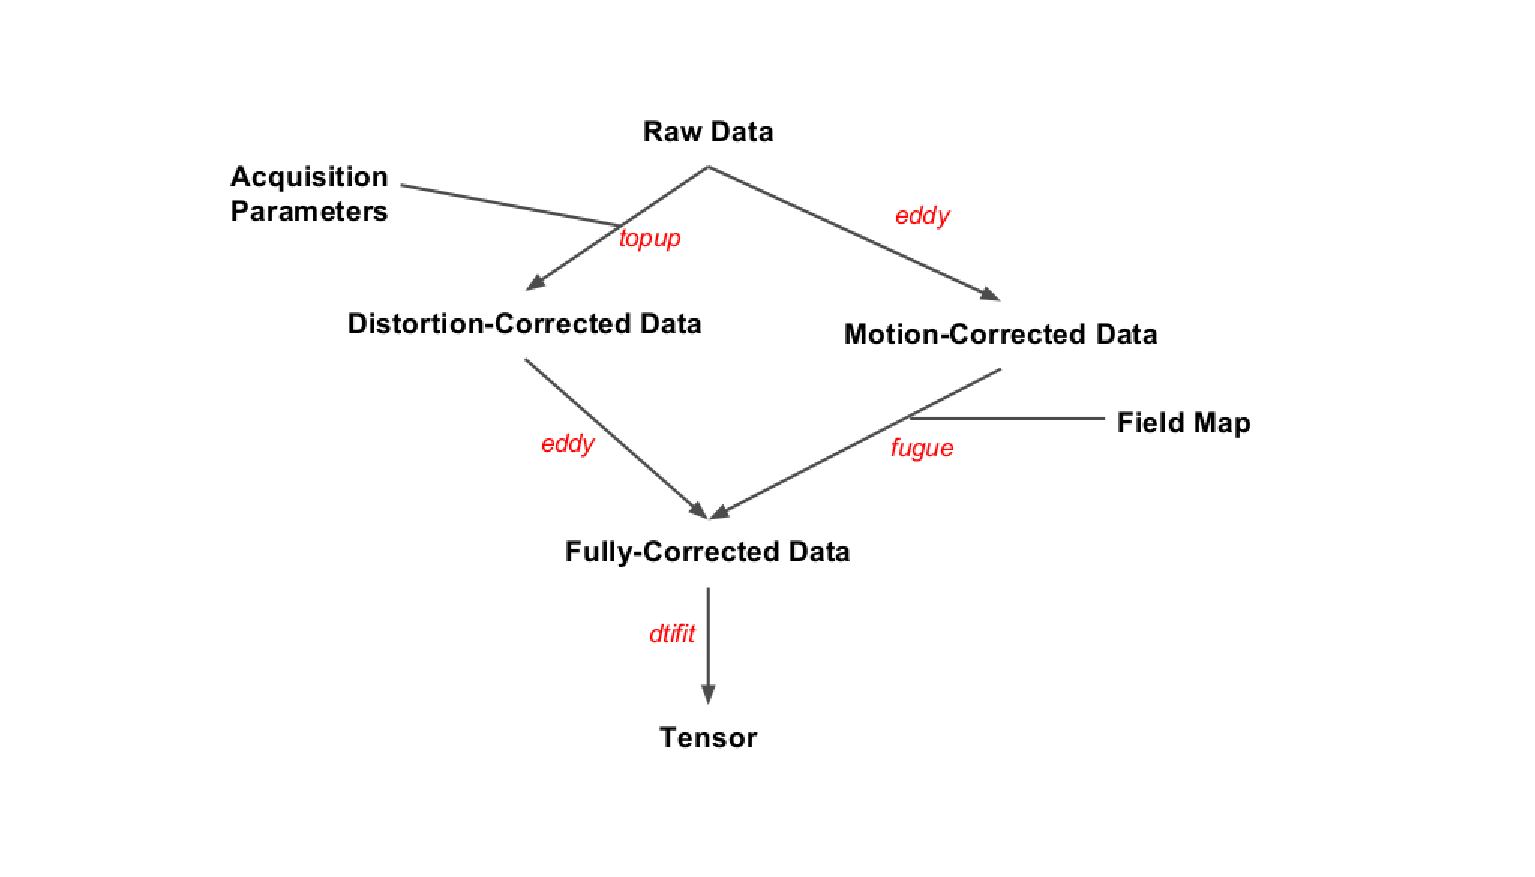
\includegraphics[width=\textwidth]{images/distcorr-flowchart.eps}
	\end{center}
	\caption{Flowchart of the Toy Makefile}
	\label{toy-example}
\end{figure}


If we were to implement this process in a \bashn{} script, the earlier
``upstream'' processes would need to be part of the conditional
block. An advantage of using \maken{} for workflows is that
\emph{only} the part that causes the ``split'' in the branching logic
needs to be surrounded by the if-then-else-end logic. Also note that
if we were using \texttt{topup} with a fieldmap, but for some reason
we wanted to do just the motion correction (like for QC, or for
debugging purposes), that unused ``branch'' of the makefile would be
available with a simple \texttt{make motion_corrected_dataset}
command. \newpage


Here's the full Makefile, located in
\texttt{dti_suceptibility_correction/subjects/fugue_DTI} and
\texttt{dti_suceptibility_correction/subjects/topup_DTI}. You can see
each of these files is in fact a symbolic link to the same file, located in
\texttt{dti_suceptibility_correction/lib/diffusion.Makefile}.

\setcounter{codehighlight}{0}
\begin{lstlisting}
	ifeq "$(origin MAKEPIPELINES)" "undefined"
	MAKEPIPELINES=/project_space/makepipelines
	endif

	PROJECT_DIR=$(MAKEPIPELINES)/dti_suceptibility_correction

	SDC_METHOD = $(shell if [ -f fieldmap.nii.gz ] ; then echo FUGUE; \
	                    elif [ -f acqparams.txt ] ; then echo TOPUP; \
	                    else echo FALSE ; fi)


	%*\lnote*NUM_DIFFUSION_VOLS =$(shell fslval raw_diffusion.nii.gz dim4 | tr -d '\040\011\012\015')


	%*\lnote*EDDY_ITERATIONS = 1
	TOPUP_MODE=fast
	ECHO_SPACING =.00072
	UNWARP_DIRECTION=y-

	.PHONY: clean tensor

	%*\lnote*mec_diffusion.nii.gz: raw_diffusion.nii.gz bval bvec brain_mask.nii.gz
		echo "0 1 0 0.072" > temp_acqparams.txt ;\
		for i in `seq 1 $(NUM_DIFFUSION_VOLS)`; do echo 1 >> temp_index.txt ; done ;\
		eddy --imain=raw_diffusion.nii.gz --mask=brain_mask.nii.gz \
			--index=temp_index.txt --acqp=temp_acqparams.txt --bvecs=bvec \
			--bvals=bval --out=mec_diffusion --niter=$(EDDY_ITERATIONS) \
			--verbose  ;\
		rm temp_acqparams.txt temp_index.txt

	%*\lnote*topup_results_movpar.txt: raw_diffusion.nii.gz acqparams.txt
		fslroi raw_diffusion.nii.gz S0_images.nii.gz 0 2 ;\
		topup --imain=S0_images --datain=acqparams.txt \
			--config=$(PROJECT_DIR)/lib/b02b0_$(TOPUP_MODE).cnf \
			--out=topup_results --fout=field_est --iout=unwarped_S0_images \
			--verbose

	ifeq ($(SDC_METHOD),TOPUP)
	sdc_mec_diffusion.nii.gz: raw_diffusion.nii.gz topup_results_movpar.txt index.txt
		eddy --imain=raw_diffusion.nii.gz --mask=brain_mask --acqp=acqparams.txt \
			--index=index.txt --bvecs=bvec --bvals=bval \
			--topup=topup_results \
			--out=sdc_mec_diffusion.nii.gz --niter=$(EDDY_ITERATIONS) \
			--verbose
		
	else ifeq ($(SDC_METHOD),FUGUE)
	sdc_mec_diffusion.nii.gz: mec_diffusion.nii.gz fieldmap.nii.gz
		fugue --loadfmap=fieldmap.nii.gz --dwell=$(ECHO_SPACING) \
			-i mec_diffusion.nii.gz -u sdc_mec_diffusion.nii.gz \
			--unwarpdir=$(UNWARP_DIRECTION) -v
	else
	$(error ERROR: neither fieldmap for FUGUE nor acquisition parameter file for TOPUP were found)
	endif

	tensor: sdc_mec_diffusion.nii.gz brain_mask.nii.gz bvec bval
		dtifit -k sdc_mec_diffusion.nii.gz -r bvec -b bval -m brain_mask -o dti

	clean:
		rm -f dti_* sdc_mec_diffusion.* mec_diffusion.* S0_images* \
		field_est.nii.gz topup_results* unwarped_S0_images.nii.gz

\end{lstlisting}


\lnum{1}\texttt{fslval} returns a trailing space as part of its output, which we pipe to \texttt{tr} for deletion.

\lnum{2}The settings here are for a quick test run for demonstration
purposes. For more accurate (but slower) processing,
\texttt{TOPUP_MODE} can be changed to 'accurate', and
\texttt{EDDY_ITERATIONS} can be increased to 5. Placing the settings
clearly in the Makefile makes it easy to extract them for quality
assurance reports. 

\lnum{3}In addition to running \texttt{eddy}, this recipe creates a simple acquisition parameters file and a simple index file (\texttt{eddy} requires that you supply one). This tells \texttt{eddy} that all the images were acquired with the phase encoding along the same direction. These files are deleted afterwards.

\lnum{4}The first two images are assumed to be the two non-diffusion weighted images (i.e. the $S _{0}$ images), with the phase encoding along different directions.


There are a few more files and commands here than in the toy example,
but the basic structure is the same. It's still missing some elements
of a full-featured DTI preprocessing pipeline (for example, unwarping
the brain mask, coregistration of the fieldmap with the diffusion
data, and rotation of the b-vectors), but this example illustrates how
using conditional statements in makefiles can make them more robust
and versatile.

\vspace{\baselineskip}
\hrule
\vspace{\baselineskip}

More information about the options and the formats of the files
supplied to \texttt{eddy}, \texttt{topup}, and \texttt{fugue} is
available on the
\href{http://fsl.fmrib.ox.ac.uk/fsl/fslwiki/FslOverview}{FSL website}.





 \clearpage \setcounter{codehighlight}{0}
\Echapter{Downloading Data From XNAT}{Karl Woelfer}{kwoelfer@uw.edu}
\label{chap:XNAT}

This is an example of how to use a Makefile to create and populate a
project directory with images from an open dataset stored in an XNAT
(eXtensible Neuroimaging Archive Toolkit) database, in this case from
the NITRC (Neuroimaging Informatics Tools and Resources Clearinghouse)
1000 Functional Connectomes project image repository at
\url{http://www.nitrc.org/ir}. The code for this example is located at \texttt{fcon_1000/Makefile}.

To run this pipeline you will need to have first created an individual
user account on NITRC, at
\url{http://www.nitrc.org/account/register.php}, and obtained access
to the 1000 Functional Connectome project.

To simplify this example, we download only a subset of the subjects in
the repository. A file with the names of these subjects is used to
determine what files to download.

In our example, we selected 23 Baltimore subjects, saved in the file \texttt{Subjects_Baltimore}.
To recreate this file you can do the following. From the NITRC Image Repository home page ``Search,'' choose Projects $\rightarrow$ 1000 Functional Connectomes. At the 1000 Functional Connectomes project home page, select Options $\rightarrow$ Spreadsheet to download a CSV file of the 1288 subjects \texttt{AnnArbor_sub00306 \ldots Taipei_sub91183}. Select a subset, or all, of the subjects from the first column of the downloaded spreadsheet, and save to a text file. 

The directory hierarchy that this Makefile creates under your project
home, from which \maken{} is run, is shown in \autoref{xnat-dir}. Note
that this Makefile assumes that the directory \texttt{visit1} 
already exists.

\begin{figure}
	\dirtree{%
		.1 fcon_1000/.
		.2 subjects/.
		.3 Baltimore_sub17017/.
		.4 visit1/.
		.5 rest.nii.gz.
		.5 T1_brain.nii.gz.
		.5 T1.nii.gz.
		.3 Baltimore_sub19738/.
		.4 visit1/.
		.5 rest.nii.gz.
		.5 T1_brain.nii.gz.
		.5 T1.nii.gz.
		.3 \ldots.
		.2 visit1/.
		.3 Baltimore_sub17017/\DTcomment{A symlink to ../subjects/Baltimore_sub17017/visit1}.
		.3 Baltimore_sub19738/.
		.3 \ldots.
	}
	\caption{XNAT access directory structure.}
	\label{xnat-dir}
\end{figure}


\begin{lstlisting}
	# Site hosting XNAT
	%*\lnote*NITRC=http://www.nitrc.org/ir3
	
	%*\lnote*SHELL=/bin/bash
	
	# Obtain the list of subjects to retrieve from NITRC
	%*\lnote*SUBJECTS = $(shell cat Subjects_Baltimore)

	%*\lnote*.PHONY: clean all allT1 allT1_brain allrest allsymlinks
\end{lstlisting}

This portion of the Makefile defines key variables and targets. 

\indent \lnum{1}We set the ``base name'' of the XNAT web site in a variable \texttt{NITRC}. This can be changed when using another XNAT repository, and the variable can be named accordingly. \\
\indent \lnum{2} By default, \maken{} uses \texttt{/bin/sh} to interpret recipes. Sometimes this can cause confusion, because \texttt{sh} has only a subset of the functionality of \texttt{bash}. We set the \maken{} variable \texttt{SHELL} explicitly. \\
\indent \lnum{3}The \texttt{SUBJECTS} variable will contain a list of the subject data we wish to download. The individual subject names will be used to create directory names. \\
\indent \lnum{4}We define six targets that do not correspond to files, so these are denoted as phony targets.

\begin{lstlisting}
	%*\lnote*all: sessionid allT1 allT1_brain allrest allsymlinks

	%*\lnote*allT1: $(SUBJECTS:%=subjects/%/visit1/T1.nii.gz)
	%*\lnote*allT1_brain: $(SUBJECTS:%=subjects/%/visit1/T1_brain.nii.gz)
	%*\lnote*allrest: $(SUBJECTS:%=subjects/%/visit1/rest.nii.gz)
	%*\lnote*allsymlinks: $(SUBJECTS:%=visit1/%)
\end{lstlisting}

\indent \lnum{5} \texttt{all} is the default target, and simply defines the five dependencies. \\
\indent \lnum{6} We need to derive the names of all the files that we
intend to create from the list of subjects. We do this using pattern
substitution to define several targets. Here, we use pattern matching
to generate a list of the T1 image names that we need to create. Each of
the subject names, e.g. \texttt{Baltimore_sub17017}, is used to create
the corresponding T1 image (e.g. \texttt{subjects/Baltimore_sub17017/visit1/T1.nii.gz}).\\
\indent \lnum{7} As above, we form the names of the skull stripped T1 images.\\
\indent \lnum{8} And the resting state images.\\
\indent \lnum{9} The last thing the Makefile does is create a
\texttt{visit1/} directory after the \texttt{subjects/} directory has
been populated. Here we use pattern matching, as above, to generate
the list of symbolic links that need to be created.  Each
\texttt{visit1/SUBJECT} directory will be a symbolic link to the actual \texttt{subjects/SUBJECTS/visit1/} directory.


\begin{lstlisting}
	%*\lnote*sessionid: 
		@echo -n "Username: " ;\
		read username ;\
		curl --user $$username $(NITRC)/REST/JSESSION > $@
\end{lstlisting}

\indent \lnum{10} Here we use the client URL Request Library
(\texttt{cURL}) to create a session with the XNAT server. The first
line prompts for the user's name on the XNAT server, the second line
reads and stores that in the variable \texttt{username}. With one
single REST transaction, the \texttt{cURL} call on the following line,
we authenticate with the XNAT server, entering a password only once,
and saving the return value \texttt{SESSIONID} in a file named
\texttt{sessionid}. This single session will persist for an
hour. Obtaining a session identifier is important to reduce load on
the remote XNAT server.
	
\begin{lstlisting}	
	%*\lnote*subjects/%/visit1/T1.nii.gz:  | sessionid
	%*\lnote*	mkdir -p `dirname $@`; \
	%*\lnote*	curl --cookie JSESSIONID=`cat sessionid` $(NITRC)/data/projects/fcon_1000/subjects/$*/experiments/$*/scans/ALL/resources/NIfTI/files/scan_mprage_anonymized.nii.gz > $@

\end{lstlisting}

\indent \lnum{11} This recipe downloads all of the T1 images required
by target \texttt{allT1} (\lnum{6}). It has an order-only dependency
upon the file \texttt{sessionid} because we assume that if these files
exist, it does not matter if they are older than the
\texttt{sessionid} file. They will only be recreated if they do not
exist. \\
\indent \lnum{12} This command creates the directory
\texttt{subjects/SUBJECT/visit1} if it does not exist (where SUBJECT
is the actual subject identifier).\\
\indent \lnum{13} This \texttt{curl} command uses the
\texttt{SESSIONID} which was stored in the \texttt{sessionid}
file. The URL defined here is specific to the location where scan data
of interest is stored on the NITRC instance of XNAT. Note that
\texttt{\$*} is used in two places to refer to the subject identifer, denoted by
\texttt{\%} in the target. The XNAT file \texttt{scan_mprage_anonymized.nii.gz} is downloaded and saved under the local name \texttt{T1.nii.gz}.

\begin{lstlisting}
	$subjects/%/visit1/T1_brain.nii.gz:  | sessionid
		mkdir -p `dirname $@`; \
		curl --cookie JSESSIONID=`cat sessionid` (NITRC)/data/projects/fcon_1000/subjects/$*/experiments/$*/scans/ALL/resources/NIfTI/files/scan_mprage_skullstripped.nii.gz > $@
\end{lstlisting}

\indent This recipe is analogous to the previous one, except
that it creates the skull stripped T1 images needed by target
\texttt{allT1_brain}.

\begin{lstlisting}
	subjects/%/visit1/rest.nii.gz:  | sessionid
		mkdir -p `dirname $@`; \
		curl --cookie JSESSIONID=`cat sessionid` $(NITRC)/data/projects/fcon_1000/subjects/$*/experiments/$*/scans/ALL/resources/NIfTI/files/scan_rest.nii.gz > $@
\end{lstlisting}

\indent Similarly, this recipe creates the resting state
images needed by \texttt{allrest}.


\begin{lstlisting}
	visit1/%:
		ln -s ../subjects/$*/visit1 $@
\end{lstlisting}

\indent  This recipe populates the project top-level \texttt{visit1/} directory with symbolic links, pointers to the actual locations of the subjects' \texttt{visit1} data downloaded above. This enables an alternate way to access the subject data.

\begin{lstlisting}
	clean:
		rm -rf subjects; \
		rm -rf visit1/*; \
		rm -f sessionid
\end{lstlisting}

This \texttt{clean} recipe will delete everything in
\texttt{subjects/}, links in the \texttt{visit1/} directory, and the
\texttt{sessionid} file.

 \clearpage \setcounter{codehighlight}{0}

%\section{Testsubject FreeSurfer}
\label{example:freesurfer}

This is an example of how to use a makefile to execute FreeSurfer in a cross-sectional context (in contrast to
\nameref{example:freesurfer}), which describes a longitudinal pipeline.  In addition, here we use FreeSurfer to
create a brain mask for skull stripping.

The code for this example is in \texttt{\$MAKEPIPELINES/testsubject/freesurfer/Makefile}.

NOTE- THIS DOES NOT QUITE MATCH THE FILE - MUST MAKE CONSISTENT.

\setcounter{codehighlight}{0} % RESET THIS BEFORE EVERY LST LISTING

\begin{lstlisting}
	ifeq "$(origin MAKEPIPELINES)" "undefined"
	MAKEPIPELINES=/project_space/makepipelines
	endif

	PROJHOME=$(MAKEPIPELINES)/testsubject 
\end{lstlisting}

This first section of the code looks to see if the environment variable
\texttt{MAKEPIPELINES} is set. This allows people who are not at IBIC
to override the default location of these files.

\begin{lstlisting}
	%*\lnote*include $(PROJHOME)/lib/makefiles/help_system.mk 

	%*\lnote*SUBJECTS=test001 

	export SUBJECTS_DIR=$(PROJHOME)/freesurfer 
	export FREESURFER_SETUP = /usr/local/freesurfer/stable5_3/SetUpFreeSurfer.sh 
	export RECON_ALL = /usr/local/freesurfer/stable5_3/bin/recon-all 
	export TKMEDIT = /usr/local/freesurfer/stable5_3/bin/tkmedit 
	QA_TOOLS=/usr/local/freesurfer/QAtools_v1.1 

	export SHELL=/bin/bash

	%*\lnote*outputstats=$(SUBJECTS:%=%/mri/aparc+aseg.mgz) $(SUBJECTS:%=%/mri/brainmask.mgz)
		$(SUBJECTS:%=%/mri/brainmask.nii.gz)

	%*\lnote*inputdirs = $(SUBJECTS:%=%)

	.PHONY: all clean qa freesurfer

	.SECONDARY: $(inputdirs) $(outputstats)
\end{lstlisting}

This portion of the Makefile defines key variables and targets. 
\lnum{1} We make use of the help system described in
\nameref{sec:practicum4}. 
\lnum{2} There is only one subject here, so for clarity we simply
write it out. However, in real life you would have many subjects, and
obtain them through a wildcard or from a file (see
\nameref{subsec:subjectlist}).
\lnum{3} We use pattern substitution to specify all of the output
targets we wish to create. These are the \texttt{aparc+aseg.mgz} file,
the \texttt{brainmask.mgz} file, and the brainmask converted to NIfTI
format (\texttt{brainmask.nii.gz}). Note that all of these files are
designated as SECONDARY targets so that they are not deleted at the end!
\lnum{4} We also use pattern substitution to set up the input directories.


\begin{lstlisting}
	 all: $(call print-help,all,Setup directories, Run Freesurfer, and Run QA) setup freesurfer qa

	 freesurfer: $(call print-help,freesurfer,Run FreeSurfer) $(outputstats)
\end{lstlisting}

The \texttt{all} and \texttt{freesurfer} targets here are documented
using the help system. 

\begin{lstlisting}
	%/mri/brainmask.mgz: %
		subj=$* ;\
		export FREESURFER_SETUP=$(FREESURFER_SETUP) ;\
		export WATERSHED_PREFLOOD_HEIGHTS='05 15 25 35' ;\
		rm -rf $${subj}/scripts/IsRunning.* ;\
		source $$FREESURFER_SETUP ;\
		export SUBJECTS_DIR=$(SUBJECTS_DIR) ;\
		recon-all  -subjid  $${subj} -multistrip -autorecon1 ;\
		height=`cat $${subj}/mri/optimal_preflood_height' ;\
		if [[ $$height == 05 ]]; then max=$$(( $$height + 5 )); WATERSHED_PREFLOOD_HEIGHTS=`echo $$height $$max'; else min=$$(( $$height - 5 )); max=$$(( $$height + 5 )); WATERSHED_PREFLOOD_HEIGHTS=`echo $$min $$height $$max'; fi ;\
		export WATERSHED_PREFLOOD_HEIGHTS ;\
		recon-all -s $${subj} -multistrip -clean-bm -gcut
\end{lstlisting}

This rule creates the brain mask (in .mgz format). We use the
\texttt{-multistrip} flag to \texttt{recon-all} which allows us to try
multiple preflood heights, trying different thresholds
automatically. Then \texttt{recon-all} is continued using the optimal
height. Note that this approach will begin a separate process
for each preflood height (e.g., four processes). This makes it a bit
hard to run this pipeline on many brains in parallel. Normally, we use
this approach when we are processing subjects one at a time after they
have been scanned.

\begin{lstlisting}
	%/mri/brainmask.nii.gz: %/mri/brainmask.mgz
		export FREESURFER_SETUP=$(FREESURFER_SETUP) ;\
		source $$FREESURFER_SETUP ;\
		mri_convert $< $@
\end{lstlisting}
This rule converts the brain mask from \texttt{mgz} format to NIfTI format.

\begin{lstlisting}
	%/mri/aparc+aseg.mgz:  %/mri/brainmask.mgz 
		subj=$* ;\
		export FREESURFER_SETUP=$(FREESURFER_SETUP) ;\
		source $$FREESURFER_SETUP ;\
		export SUBJECTS_DIR=$(SUBJECTS_DIR) ;\
		recon-all -s $${subj} -autorecon2 -autorecon3 
\end{lstlisting}

This rule finishes the remaining stages of
\texttt{recon-all}. It depends upon the brain mask being generated
(the result of the previous rule).

\begin{lstlisting}
	 setup: $(call print-help,setup,Setup subject directories) $(inputdirs) 

	%:  $(PROJHOME)/%/T1.nii.gz 
		mkdir -p $@/mri/orig; \
		cp $^ $@/mri/orig; \
		cd $@/mri/orig; \
		mri_convert *nii.gz 001.mgz 
\end{lstlisting}

The \texttt{setup} target depends upon the T1 image in the subject
directory (here, in \texttt{\$PROJHOME}). It creates a FreeSurfer
style subject directory, copies the file there, and converts it to
NIfTI format. 

\begin{lstlisting}
	qa: $(call print-help,qa, Run QA - do this interactively with screensaver shut off) $(inputdirs:%=QA/%)

QA/%: %
	source $(FREESURFER_SETUP) ;\
	$(QA_TOOLS)/recon_checker -s $*
\end{lstlisting}

We run the FreeSurfer QA tools to generate images that we can put into
our own reports. One problem with QA is that the images cannot be
generated in parallel in batch. We include a warning in the help
system that they should be generated interactively without a
screensaver. 

\begin{lstlisting}
clean:
	echo rm -rf $(inputdirs)
\end{lstlisting}

Finally, we define a \texttt{clean} target to remove all processing
results. 
\clearpage
%\ input{testsubject-Makefile-example.tex} \clearpage
%\section{Testsubject Transformations}
\def\sectionautorefname{Testsubject Transformations}
\label{sec:testsubjectxfm}

This is an example of using a makefile to create a set of transformation matrices using different registration methods available in FSL. 

The code for this example is in \texttt{\$MAKEPIPELINES/testsubject/lib/makefiles/xfm.mk}. It is included by \texttt{\$MAKEPIPELINES/testsubject/test001/Makefile}. Therefore, certain variables that this example uses are defined there. This approach helps to organize multiple makefiles and reuse rules across projects.

\setcounter{codehighlight}{0} % RESET THIS BEFORE EVERY LST LISTING
\begin{lstlisting}
	.PHONY=clean_transform tranforms 

	transforms:  $(call print-help,xfm,Create resting state to MNI transformations) xfm_dir xfm_dir/MNI_to_rest.mat
\end{lstlisting}

The first line defines two phony targets (clean\_transform and transforms). The \texttt{.PHONY} target can be set as many times as you need to, and note that each makefile included by \texttt{testsubject/test001/Makefile} defines phony targets. 

The second target, \texttt{xfm}, uses the \texttt{print-help} call introduced in \autoref{sec:practicum4} to document this main function, to create an MNI to resting state transformation.

\begin{lstlisting}
	xfm_dir:
	%*\lnote*	mkdir -p xfm_dir

	%*\lnote*xfm_dir/T1_to_MNI.mat: xfm_dir T1_skstrip.nii.gz 
		flirt -in T1_skstrip.nii.gz -ref $(STD_BRAIN) -omat $@
\end{lstlisting}

\lnum{1} We define a target to create a directory, \texttt{xfm_dir},
to hold all of our transformations. This handy because it allows us to
reuse transformations for other analyses. We know that
the registrations saved here will be checked. 

\lnum{2} This is just a simple rule to call \texttt{flirt} to perform
linear registration of the skull stripped T1 image to the standard
brain. Note that the definition for \texttt{STD_BRAIN} comes from the
including makefile, as do the rules to create the file \texttt{T1_skstrip.nii.gz}.

\begin{lstlisting}
	rest_dir/rest_mc_vol0.nii.gz: rest_dir/rest_mc.nii.gz
		fslroi $< $@ 0 1

	xfm_dir/rest_to_T1.mat: rest_dir/rest_mc_vol0.nii.gz T1_skstrip.nii.gz
		mkdir -p xfm_dir ;\
		%*\lnote*epi_reg --epi=rest_dir/rest_mc_vol0.nii.gz --t1=T1.nii.gz --t1brain=T1_skstrip.nii.gz --out=xfm_dir/rest_to_T1
\end{lstlisting}

These rules use FSL's \texttt{epi_reg} program to register the resting
state data to the subject's structural data. We noticed that
\texttt{epi_reg} used a lot of memory when running, limiting the
number of processors that we could use in parallel to preprocess
resting state data. \lnum{3} This requirement can be circumvented by using only
the first volume of the resting state data, obtained in the first
rule. 


\begin{lstlisting}
	xfm_dir/T1_to_rest.mat: xfm_dir/rest_to_T1.mat
		convert_xfm -omat $@ -inverse $<

	xfm_dir/MNI_to_T1.mat: xfm_dir/T1_to_MNI.mat
		convert_xfm -omat $@ -inverse $<

	xfm_dir/MNI_to_rest.mat:  xfm_dir/T1_to_rest.mat xfm_dir/MNI_to_T1.mat
		convert_xfm -omat xfm_dir/MNI_to_rest.mat -concat xfm_dir/T1_to_rest.mat  xfm_dir/MNI_to_T1.mat
\end{lstlisting}
We obtain the T1 to resting matrix by inverting the resting to T1
matrix, and similarly for the MNI to T1 matrix. Finally, these
matrices are concatenated to create the final target,
\texttt{MNI_to_rest.mat}. Notice that everything else we needed was
automatically created as necessary to make this final target.


\begin{lstlisting}
	clean_transform: 
		rm -rf  xfm_dir 
\end{lstlisting}
Finally, we define a target to remove what we have created and clean
up. Notice that we call it \texttt{clean_transform}, rather than simply
\texttt{clean}, so that it does not override any other targets for
cleaning up that are included by the including Makefile.  \clearpage
%\section{Testsubject QA Makefile}
\label{example:testsubjectQA}

This is an example of using a makefile to create quality assurance (QA) images, and then generate a final QA report in HTML using R Markdown. 

The code for this example is in \texttt{testsubject/lib/makefiles/QA.mk}, and it is included by\linebreak \texttt{testsubject/test001/Makefile}.

\setcounter{codehighlight}{0} % RESET THIS BEFORE EVERY LST LISTING
\begin{lstlisting}
	%*\lnote*NIPYPATH=/usr/local/anaconda/bin
	FSL_DIR=/usr/share/fsl/5.0

	%*\lnote*.PHONY: TNSR MotionGraphs SkullstripQA QAReport

	%*\lnote*qa:   $(call print-help, qa, Create QA report) TSNR MotionGraphs SkullstripQA QAreport
\end{lstlisting}

\noindent\lnum{1} As is customary in a makefile, we first define paths
to locations that we want to refer to later on. \\
\lnum{2} Here, our phony targets are targets that are not actual files.\\
\lnum{3} This line tells the \maken{} help system what to do when you
are unsure of what this makefile does. Here, it will print out what
the \texttt{qa} target does (i.e., create a QA report). See \nameref{sec:practicum4} for more information about the help system. \\

\begin{lstlisting}
	%*\lnote*TSNR: QA/images/rest_tsdiffana.gif

	QA/images/%_tsdiffana.gif: rest.nii.gz
		%*\lnote*mkdir -p QA/images ;\
		%*\lnote*pngout=`echo $@|sed 's/gif/png/g'` ;\
		%*\lnote*$(NIPYPATH)/nipy_tsdiffana --out-file $$pngout $< ;\
		convert $$pngout $@ ;\
		rm -f $$pngout
\end{lstlisting}

\noindent\lnum{4} Our first target creates TSNR images for the QA. In this example, the phony target TSNR only wants \maken{} to create a single \texttt{gif} image. \\
\lnum{5} This line creates a directory called \texttt{QA/images} if it does not already exist. The \texttt{-p} flag tells \texttt{mkdir} not to throw an error if that directory exists, but create it if it does not.
\lnum{6} The variable \texttt{pngout} is defined to take the filename of your target and substitute \texttt{gif} with \texttt{png}.\\
\lnum{7} Subsequently, the code calls the script \texttt{nipy\_tsdiffana} which is located in the directory \texttt{\$(NIPYPATH)} you defined earlier.\\ The python script will generate a \texttt{png} image comprised of 4 graphs showing the scaled variance, slice-by-slice variance, scaled mean voxel intensity and the max/mean/min slice variation of your resting-state time series, as seen in the image below. \\

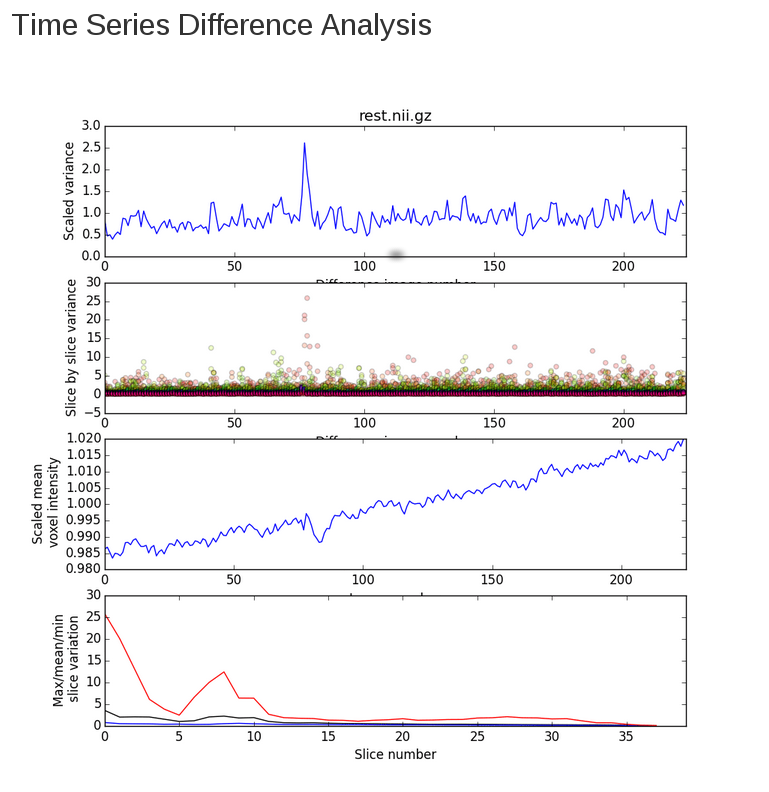
\includegraphics[scale=0.5]{images/QAtsdiffana.png}

\begin{lstlisting}
	MotionGraphs: QA/images/rest_MotionGraphRotations.gif 

	QA/images/rest_MotionGraphRotations.gif: rest_dir/rest_mc.nii.gz
		%*\lnote*$(PROJECT_HOME)/bin/R/MakingGraphs.Rscript  QA/images rest
\end{lstlisting}

\lnum{8}  \texttt{MakingGraphs.Rscript} is a R script that will generate 4 separate graphs for you: \\
	\tab 1. A motion rotations graph showing rotations along the x/y/z planes.\\
	\tab 2. A motion translations graph showing translations along the x/y/z planes.\\
	\tab 3. A framewise displacement (FD) graph to show displacement in mm across acquired volumes.\\
	\tab 4. A signal intensity (DVARS) graph to show signal intensity across acquired volumes.\\
	To understand the usage of an R script, it is usually necessary to look at the code itself. In this line, the R script called with the output directory \texttt{QA/images} as the first argument, followed by the prefix \texttt{rest} to be used for naming the output images.\\

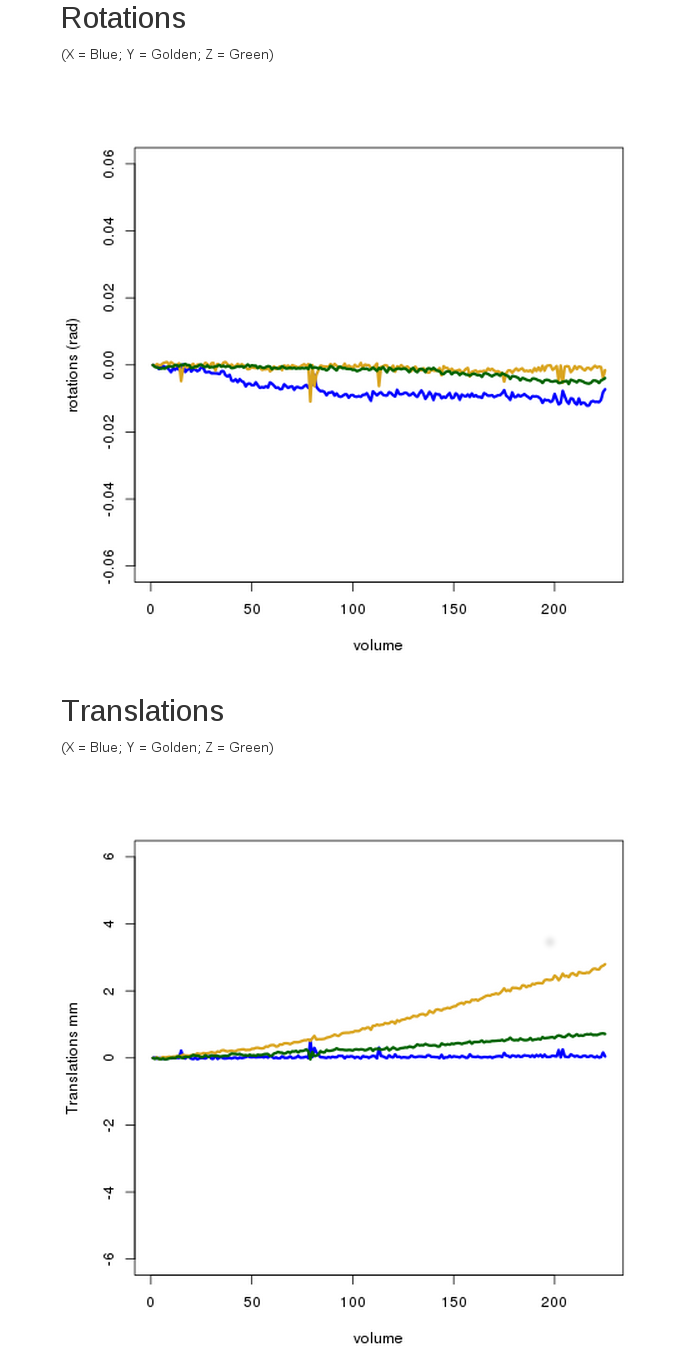
\includegraphics[scale=0.3]{images/QAmotion1.png}
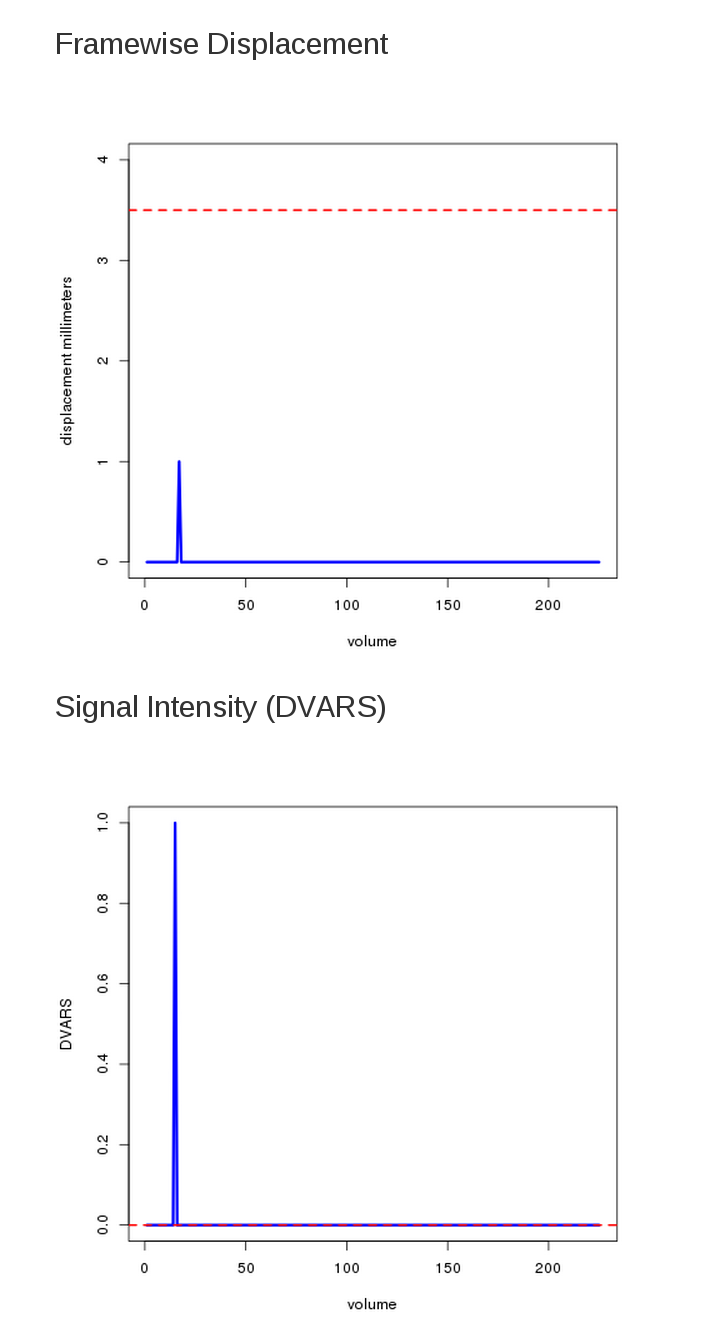
\includegraphics[scale=0.3]{images/QAmotion2.png}

\begin{lstlisting}
	SkullstripQA: QA/images/T1_skstrip.gif

	QA/images/T1_skstrip.gif: T1.nii.gz T1_skstrip_mask.nii.gz
		mkdir -p QA/images ;\
		%*\lnote*$(FSL_DIR)/bin/overlay 1 1 $< -a $(word 2,$^) 1 10 rendered_T1_brain.nii.gz ;\
		%*\lnote*$(PROJECT_HOME)/bin/slices rendered_T1_brain.nii.gz -o `dirname $@`/`basename $@ .gif`.png ;\
		%*\lnote*convert `dirname $@`/`basename $@ .gif`.png -resize 500 $@ ;\
		rm rendered_T1_brain.nii.gz ;\
		rm `dirname $@`/`basename $@ .gif`.png

\end{lstlisting}


To ensure that our skull-strip does not remove too much of the brain or too little of the skull, we can create an image to overlay the skull-stripped mask generated from \texttt{resting.mk} on top of the T1 brain. \\
\tab\lnum{9} FSL \texttt{overlay} is a tool that is used to overlay a 3D images over another. It is capable of overlaying a maximum of 2 images on top of a reference image. Type \texttt{overlay} into your command line to understand how it is used. In this line, we call \texttt{overlay}. The \texttt{1}s that are provided as arguments specify the color and output type of your overlay. The next argument is the background image, which in this case is the first dependency we have listed, i.e. \texttt{T1.nii.gz}. The \$\textasciicircum{} refers to this file. The final output image is called \texttt{rendered\_T1\_brain.nii.gz}. Again, to understand the flags, you must look at overlay's usage. \\
\lnum{10} FSL \texttt{slices} is a script that calls the FSL tool \texttt{slicer} to create an image consisting of 3 axial, 3 sagittal and 3 coronal slices. Here, we feed it the \texttt{rendered\_T1\_brain.nii.gz} file that we want FSL \texttt{slices} to use. The output will be a file called \texttt{QA/images/T1\_skstrip.png}. Instead of typing out the full name of the file, however, we simply provide the directory name and basename of our target and replace \texttt{.gif} with \texttt{.png}. \\
\lnum{11} Following this, we convert our PNG image into a GIF image, using ImageMagick's \texttt{convert} that performs the conversion and resizes the image.\footnote{This step was necessary in earlier versions of R Markdown that had trouble including PNG images, but may not be necessary for you.}\\

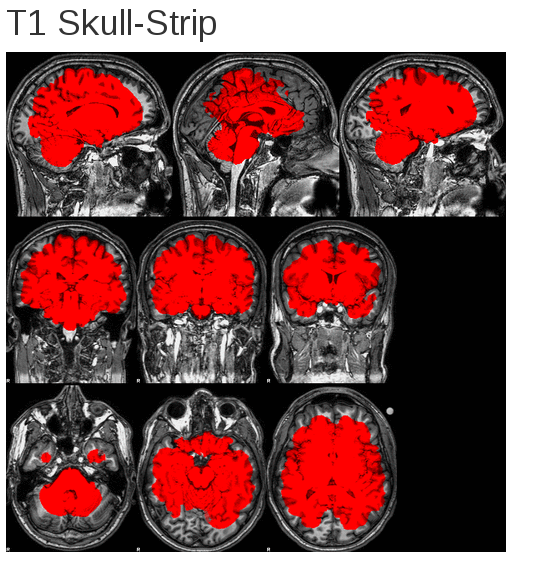
\includegraphics[scale=0.4]{images/QAskullstrip.png}

\begin{lstlisting}
	QAreport: QA/rest_Preprocessing.html 

	QA/rest_Preprocessing.html: $(PROJECT_HOME)/lib/Rmd/fMRI.Rmd TSNR MotionGraphs SkullstripQA
		%*\lnote*sed -e 's/SUBJECT/$(subject)/g' -e 's/TASK/rest/g' $(word 1,$^) > QA/rest_Preprocessing.Rmd ;\
		%*\lnote*R -e 'library("rmarkdown");rmarkdown::render("QA/rest_Preprocessing.Rmd")' ;\
		rm -f QA/rest_Preprocessing.Rmd QA/rest_Preprocessing.md
\end{lstlisting}


Finally, to generate our QA HTML report, we use R Markdown. We do this by writing a file called \texttt{fMRI.Rmd}, which is the first dependency listed here. The \texttt{fMRI.Rmd} file reads the QA images that were generated in the previous portions of this makefile to create a HTML page (see \nameref{sec:practicum4} for a brief explanation of what goes into a Rmd file and how to write one). \\
\lnum{12} In this line, we substitute pattern strings in the \texttt{fMRI.Rmd} file with variables that have been defined in the makefiles by using \texttt{sed}. \texttt{SUBJECT}, for instance, will be replaced with the \texttt{\$(subject)} variable defined in the main makefile \texttt{\$(PROJECT\_HOME)/test001/Makefile}. \texttt{TASK} will be replaced with \texttt{rest}, because we are only interested in looking at the QA report for resting-state functional scans for now. We can define another variable called \texttt{task} if we have several types of runs that we want to generate QA reports for (e.g., task runs or multiple resting state runs). Once the pattern strings have been substituted, the \texttt{fMRI.Rmd} file will be copied over to the \texttt{QA} directory and be renamed as \texttt{rest\_Preprocessing.Rmd}. \\
\lnum{13} This line tells R to load the `\texttt{rmarkdown}' library so that it can read the R Markdown file. R will then render \texttt{QA/rest\_Preprocessing.Rmd} to create your HTML report! \\

To view the full report, you can open the file \texttt{testsubject/test001/QA/rest_Preprocessing_example.html} in a browser.


\begin{lstlisting}
		clean_qa: 
		rm -rf QA
\end{lstlisting}

Finally, with other makefiles, we define a \texttt{clean} target specifically for QA. Because quality assurance is an intermediate step in the neuroimaging processing pipeline, we do not necessarily need to retain the QA images and reports once they have been checked.


 \clearpage
